\documentclass[11pt,a4paper]{article}

\usepackage[utf8]{inputenc}
\usepackage[T1]{fontenc}
\usepackage{amsmath,amssymb}
\usepackage{graphicx}
\usepackage{booktabs}
\usepackage{longtable}
\usepackage{geometry}
\usepackage{hyperref}
\usepackage{xcolor}
\usepackage{enumitem}
\usepackage{float}
\usepackage{siunitx}
\usepackage[version=4]{mhchem}
\usepackage{tikz}
\usetikzlibrary{arrows.meta,positioning,shapes.geometric,calc}
\usepackage{tcolorbox}
\usepackage{fancyhdr}
\usepackage{titlesec}

\geometry{margin=2.5cm}

% Custom colors
\definecolor{evalcolor}{RGB}{0,100,0}
\definecolor{evalbox}{RGB}{230,245,230}
\definecolor{warncolor}{RGB}{180,60,0}
\definecolor{warnbox}{RGB}{255,240,230}
\definecolor{threshcolor}{RGB}{0,50,120}
\definecolor{threshbox}{RGB}{230,240,255}

% Custom evaluation box
\newtcolorbox{evaluation}{
  colback=evalbox,
  colframe=evalcolor,
  title={\textbf{Computational Chemistry Evaluation}},
  fonttitle=\color{white},
  colbacktitle=evalcolor,
  boxrule=0.5pt,
  arc=3pt,
}

% Warning/concern box
\newtcolorbox{concern}{
  colback=warnbox,
  colframe=warncolor,
  title={\textbf{Potential Concern}},
  fonttitle=\color{white},
  colbacktitle=warncolor,
  boxrule=0.5pt,
  arc=3pt,
}

% Threshold summary box
\newtcolorbox{threshbox}{
  colback=threshbox,
  colframe=threshcolor,
  title={\textbf{Key Thresholds}},
  fonttitle=\color{white},
  colbacktitle=threshcolor,
  boxrule=0.5pt,
  arc=3pt,
}

\pagestyle{fancy}
\fancyhf{}
\fancyhead[L]{\small CRN-Cloud PES Exploration Algorithm}
\fancyhead[R]{\small \thepage}
\fancyfoot[C]{\small Internal Documentation -- \today}

\title{\textbf{CRN-Cloud: Potential Energy Surface Exploration Algorithm} \\[0.5em]
\large A Detailed Technical Report for Computational Chemistry Review}
\author{Auto-generated from source code analysis}
\date{\today}

\begin{document}

\maketitle
\tableofcontents
\newpage

%=============================================================================
\section{Executive Summary}
%=============================================================================

This document describes the Potential Energy Surface (PES) exploration algorithm implemented in the CRN-Cloud codebase. The algorithm discovers local minima (stable conformers) and first-order saddle points (transition states) on the PES of a given molecule, using a machine-learned (ML) force field as the energy/force/Hessian provider.

The overall strategy is:
\begin{enumerate}
    \item Start from an initial molecular geometry, relax it to a local minimum.
    \item Run molecular dynamics (MD) from that minimum to sample configuration space.
    \item Extract candidate geometries from the MD trajectory.
    \item Optimize each candidate toward a first-order saddle point using Partitioned Rational Function Optimization (P-RFO).
    \item Validate each saddle point by displacing along the imaginary mode and relaxing both directions to minima.
    \item Add new minima and transition states (TSs) to a graph, with deduplication.
    \item Repeat from the next unexplored minimum until all minima are explored.
\end{enumerate}

\begin{evaluation}
The overall workflow follows established computational chemistry practices: MD sampling to escape local basins, saddle-point optimization via eigenvector following, and IRC-like validation of transition states. This is conceptually similar to approaches used in programs like \texttt{AutoMeKin}, \texttt{KinBot}, or the nanoreactor approach. The key difference here is that \textbf{all energy evaluations use an ML force field} (MACE-type), not DFT or semi-empirical methods. This makes the algorithm orders of magnitude faster but introduces questions about the reliability of the PES description---especially for barrier heights and Hessian eigenvalues, which ML models are typically less accurate at predicting than equilibrium properties.
\end{evaluation}


%=============================================================================
\section{Algorithm Overview: The Main Loop}
\label{sec:main-loop}
%=============================================================================

The entry point is the function \texttt{explore\_pes()} (file: \texttt{pes\_explorer.py}). The algorithm proceeds as follows:

\subsection{Step 0: Initialization}

\begin{enumerate}
    \item The input molecular geometry (as an ASE \texttt{Atoms} object) is \textbf{relaxed to a local minimum} using trust-region Newton optimization (see Section~\ref{sec:minimization}).
    \item A \texttt{PESGraph} object is created. This is a graph data structure (backed by NetworkX) where:
    \begin{itemize}
        \item \textbf{Nodes} = local minima (conformers)
        \item \textbf{Edges} = transition states connecting pairs of minima
    \end{itemize}
    \item The relaxed initial structure is added as the first minimum (MIN-0).
    \item A random seed is set for reproducibility (default: 42).
\end{enumerate}

\subsection{Step 1: Select the Next Minimum to Explore}

At each iteration, the algorithm selects the \textbf{lowest-energy unexplored minimum} from the graph:
\begin{equation}
    \text{MIN}_\text{next} = \arg\min_{m \in \mathcal{M}_\text{unexplored}} E(m)
\end{equation}

\begin{threshbox}
\begin{itemize}
    \item \textbf{Maximum iterations:} 200 (configurable; in production often set to 10 via \texttt{PES\_MAX\_ITERATIONS} environment variable).
    \item \textbf{Termination:} The loop stops when either all minima have been explored or the maximum number of iterations is reached.
\end{itemize}
\end{threshbox}

\begin{evaluation}
Exploring the lowest-energy minimum first is a reasonable heuristic: lower-energy conformers are more thermodynamically relevant and more likely to be kinetically accessible. However, this strategy has a bias---it will preferentially explore the most stable part of the PES and may miss high-energy but kinetically important pathways. An alternative would be Boltzmann-weighted sampling or exploration based on connectivity (exploring minima with fewer known connections first). For the purpose of building a reaction network, this lowest-energy-first approach is defensible because reactions with the lowest barriers (most kinetically relevant) tend to involve the most stable intermediates.
\end{evaluation}

\subsection{Step 2: Molecular Dynamics Sampling}

From the selected minimum, an MD simulation is run to sample the PES around it (see Section~\ref{sec:md}).

\subsection{Step 3: TS Candidate Selection}

Frames from the MD trajectory are selected as starting points for transition state optimization (see Section~\ref{sec:ts-sampling}).

\subsection{Step 4: Saddle Point Optimization}

Each candidate is optimized toward a first-order saddle point using P-RFO (see Section~\ref{sec:prfo}).

\subsection{Step 5: Transition State Validation}

Converged saddle points are validated by displacing along the imaginary mode and relaxing both directions (see Section~\ref{sec:ts-validation}).

\subsection{Step 6: Deduplication and Graph Update}

New minima and TSs are deduplicated against existing entries and added to the graph (see Section~\ref{sec:dedup}).

\subsection{Step 7: Mark as Explored and Continue}

The current minimum is marked as ``explored'' and the loop returns to Step~1.


%=============================================================================
\section{Molecular Dynamics Sampling}
\label{sec:md}
%=============================================================================

The MD simulation is run using ASE's built-in integrators. The purpose is \textbf{not} to simulate kinetics, but to efficiently sample configuration space around a minimum---to generate geometries that lie on or near reaction pathways departing from that minimum.

\subsection{MD Parameters}

\begin{threshbox}
\begin{tabular}{lrl}
\toprule
Parameter & Default & Description \\
\midrule
\texttt{md\_steps} & 2500 & Number of MD steps \\
\texttt{md\_step\_size\_fs} & \SI{0.5}{fs} & Integration timestep \\
\texttt{temperature} & \SI{300}{K} & Target temperature \\
\texttt{thermostat} & Langevin & Type of thermostat \\
\texttt{thermostat\_tau} & \SI{100}{fs} & Thermostat coupling time constant \\
\texttt{md\_save\_interval} & 10 & Save snapshot every $N$ steps \\
\bottomrule
\end{tabular}
\end{threshbox}

\noindent With these defaults, the total simulation time is $2500 \times 0.5 = \SI{1250}{fs} = \SI{1.25}{ps}$, producing approximately $2500/10 = 250$ saved snapshots.

\subsection{Thermostat Details}

The Langevin thermostat adds stochastic friction:
\begin{equation}
    m_i \ddot{\mathbf{r}}_i = \mathbf{F}_i - \gamma m_i \dot{\mathbf{r}}_i + \sqrt{2 \gamma m_i k_B T}\, \boldsymbol{\xi}(t)
\end{equation}
where $\gamma = 1/\tau$ is the friction coefficient (with $\tau = \SI{100}{fs}$) and $\boldsymbol{\xi}(t)$ is Gaussian white noise. Initial velocities are drawn from a Maxwell--Boltzmann distribution at the target temperature.

\begin{evaluation}
The Langevin thermostat is appropriate for PES exploration because it ensures good ergodic sampling. The coupling time of \SI{100}{fs} is moderately tight, which helps maintain the target temperature and prevents the system from accumulating too much kinetic energy in any single mode. The short simulation time (\SI{1.25}{ps}) is justified because the goal is not to observe reactive events but merely to visit a diverse set of geometries near the minimum. However, at \SI{300}{K}, the system has $k_BT \approx \SI{0.026}{eV}$, so it will primarily sample low-energy regions. Higher-barrier pathways ($> \SI{0.5}{eV}$) will almost never be sampled directly by the MD. This is intentional---the P-RFO optimizer (Section~\ref{sec:prfo}) will walk from nearby geometries up to the saddle point.

\textbf{Potential concern:} A \SI{0.5}{fs} timestep is safe for most organic molecules (the fastest vibrations, C--H stretches, have periods of $\sim$\SI{10}{fs}), but could be marginal for systems with very light atoms (e.g., bare H atoms after bond dissociation) or for highly strained geometries encountered during exploration. The ML force field's smoothness mitigates this somewhat.
\end{evaluation}


%=============================================================================
\section{Transition State Candidate Selection}
\label{sec:ts-sampling}
%=============================================================================

After MD, frames from the trajectory are selected as starting points for saddle point optimization.

\subsection{Random Sampling (Default)}

By default (\texttt{use\_saddle\_metric = False}), \textbf{32 frames are selected uniformly at random} from the trajectory. This is simple but effective because the P-RFO optimizer is robust enough to converge from diverse starting points.

\subsection{Saddle Metric (Optional)}

If enabled, a heuristic score is computed for each frame:
\begin{equation}
    S_i = \hat{E}_i - \hat{F}_i - 2\hat{M}_i
\end{equation}
where $\hat{E}$, $\hat{F}$, $\hat{M}$ are min-max normalized energy, force norm, and momentum norm respectively (after low-pass Butterworth filtering with cutoff frequency 0.05 and order 2). Frames with the highest scores are selected (top 10th percentile), then randomly subsampled to 32.

The intuition: near a transition state, the energy is high (large $\hat{E}$), forces are small (low $\hat{F}$, because the gradient vanishes at a stationary point), and momenta are low (the system slows down as it passes through the saddle). The factor of 2 on momenta gives extra weight to the ``slowing down'' criterion.

\begin{threshbox}
\begin{tabular}{lrl}
\toprule
Parameter & Default & Description \\
\midrule
\texttt{n\_ts\_samples} & 32 & Number of candidates to extract \\
\texttt{use\_saddle\_metric} & False & Use heuristic scoring vs.\ random \\
\texttt{ts\_top\_percentile} & 10\% & Percentile for saddle metric selection \\
\texttt{filter\_cutoff} & 0.05 & Butterworth filter cutoff \\
\texttt{filter\_order} & 2 & Butterworth filter order \\
\bottomrule
\end{tabular}
\end{threshbox}

\begin{evaluation}
Random sampling is actually a reasonable default here. The saddle metric is a heuristic with no formal justification, and in practice, the P-RFO optimizer converges to saddle points from a wide range of starting geometries---the starting point doesn't need to be especially close to a TS. The decision to use random sampling by default suggests that in testing, the saddle metric did not substantially improve results.

One subtlety: selecting 32 candidates from 250 frames means about 13\% of frames are used. This is generous and ensures good coverage. Each candidate will be independently optimized, so redundant starting points (which converge to the same TS) are handled by deduplication later.
\end{evaluation}


%=============================================================================
\section{Saddle Point Optimization (P-RFO)}
\label{sec:prfo}
%=============================================================================

The Partitioned Rational Function Optimization (P-RFO) algorithm is used to walk each candidate geometry toward a first-order saddle point. This is a well-established method in computational chemistry (Banerjee et al., 1985; Baker, 1986).

\subsection{Mathematical Foundation}

At each step, the algorithm:
\begin{enumerate}
    \item Computes the energy $E$, forces $\mathbf{f} = -\nabla E$, and full Hessian $\mathbf{H}$ using the ML force field.
    \item \textbf{Projects out} the 6 trivial modes (3 translations + 3 rotations) from the Hessian:
    \begin{equation}
        \mathbf{H}_\text{proj} = \mathbf{P} \mathbf{H} \mathbf{P}
    \end{equation}
    where $\mathbf{P} = \mathbf{I} - \sum_{k=1}^{6} \mathbf{v}_k \mathbf{v}_k^\top$ and $\{\mathbf{v}_k\}$ are mass-weighted orthonormal translation/rotation vectors obtained via Gram--Schmidt orthonormalization.
    \item Diagonalizes the projected Hessian:
    \begin{equation}
        \mathbf{H}_\text{proj} = \sum_i \lambda_i \mathbf{u}_i \mathbf{u}_i^\top
    \end{equation}
    \item Transforms the gradient $\mathbf{g} = -\mathbf{f}$ into the eigenvector basis: $g_i = \mathbf{u}_i \cdot \mathbf{g}$.
    \item Computes the step in each mode using the augmented Hessian RFO formulation. For each mode $i$, the step component is:
    \begin{equation}
        p_i = \frac{\mu_i}{g_i}, \qquad \mu_i = \frac{\lambda_i \pm \sqrt{\lambda_i^2 + 4g_i^2}}{2}
    \end{equation}
    where $+$ is used for the \textbf{TS mode} (maximization direction---walk \emph{uphill}) and $-$ for all other modes (minimization---walk \emph{downhill}).
\end{enumerate}

\subsection{Mode Following}

The algorithm tracks which eigenvector corresponds to the TS mode across steps. At the first step, the \textbf{lowest eigenvalue mode} is selected. In subsequent steps, the mode with the \textbf{best overlap} with the previous TS mode eigenvector is followed:
\begin{equation}
    i_\text{TS} = \arg\max_i \left| \mathbf{u}_i \cdot \mathbf{u}_\text{TS}^{(\text{prev})} \right|
\end{equation}
This prevents the optimizer from ``jumping'' between different modes when eigenvalues cross.

\subsection{Trust Region}

The step is constrained by \textbf{partitioned trust radii}:
\begin{itemize}
    \item \textbf{TS mode trust radius:} Maximum step along the TS mode direction (default: $1.5 \times$ min trust radius).
    \item \textbf{Minimization trust radius:} Maximum step in the orthogonal subspace.
\end{itemize}

After computing the step, the algorithm:
\begin{enumerate}
    \item Evaluates the trial position's energy.
    \item Computes the trust region ratio: $\rho = \Delta E_\text{actual} / \Delta E_\text{predicted}$, where
    \begin{equation}
        \Delta E_\text{predicted} = -\mathbf{f} \cdot \mathbf{p} + \frac{1}{2} \mathbf{p}^\top \mathbf{H} \mathbf{p}
    \end{equation}
    \item If $\rho > 0.1$ (accept threshold), the step is accepted.
    \item If $\rho < 0.1$, the trust radius is halved and the step is retried (up to 5 retries).
    \item After acceptance, the trust radii are adapted:
    \begin{itemize}
        \item $\rho < 0.25$ or $\rho > 2.0$: Shrink by factor 0.5 (model is poor).
        \item $0.5 < \rho < 1.5$: Expand by factor 1.5 if the step hit the trust boundary (model is good).
    \end{itemize}
\end{enumerate}

\subsection{Convergence Criteria}

\begin{threshbox}
\begin{tabular}{lrl}
\toprule
Parameter & Default & Description \\
\midrule
\texttt{ts\_max\_steps} & 120 & Maximum optimization steps \\
\texttt{ts\_force\_tol} & \SI{0.01}{eV/\angstrom} & Max force component tolerance \\
Trust radius (initial) & \SI{0.5}{\angstrom} & Initial trust region \\
Trust radius (min) & \SI{0.01}{\angstrom} & Minimum trust region \\
Trust radius (max) & \SI{0.3}{\angstrom} & Maximum trust region \\
TS trust scale & 1.5 & TS mode gets $1.5\times$ trust radius \\
Step accept threshold & 0.1 & Min.\ $\rho$ to accept step \\
Max step retries & 5 & Retries per step \\
\bottomrule
\end{tabular}
\end{threshbox}

A saddle point is declared \textbf{converged and first-order} when:
\begin{enumerate}
    \item $\max_i |f_i| < \SI{0.01}{eV/\angstrom}$ \textbf{and} $f_\text{RMS} < \SI{0.005}{eV/\angstrom}$ (forces are small),
    \item The projected Hessian has \textbf{exactly one negative eigenvalue} (first-order saddle point).
\end{enumerate}

\subsection{Early Stopping}

The optimizer also detects pathological behavior:
\begin{itemize}
    \item \textbf{Stuck:} Over the last 20 steps, both net displacement and total path length are below $10^{-4}$~\AA.
    \item \textbf{Oscillating:} Net displacement / path length $< 0.1$ (the optimizer is going back and forth).
    \item \textbf{Bad steps:} More than 20 consecutive steps with $\rho < 0.1$ or $\rho > 2.0$ at minimum trust radius.
\end{itemize}

\begin{evaluation}
The P-RFO implementation is textbook-correct and includes several important practical refinements: mode-following, partitioned trust radii, and early stopping. The force tolerance of \SI{0.01}{eV/\angstrom} is appropriate for ML force fields---tighter convergence would be meaningless given the model's intrinsic uncertainty (typically \SI{0.01}--\SI{0.05}{eV/\angstrom} in forces).

\textbf{Important chemical consideration:} The requirement for exactly one negative eigenvalue is the correct criterion for a first-order saddle point (transition state). However, this check is only as reliable as the Hessian from the ML model. ML Hessians can have spurious small negative eigenvalues (especially for floppy modes like methyl rotations or ring puckering), which would cause a true TS to be rejected as ``second-order.'' Conversely, a very flat PES region might show zero negative eigenvalues even though a nearby true TS exists. The zero-mode threshold of $5 \times 10^{-3}$~eV/\AA$^2$ for ``significant'' eigenvalues helps mitigate this, but practitioners should be aware that borderline cases may be misclassified.

The trust region approach with the predicted/actual energy ratio ($\rho$) is standard and robust. The accept threshold of $\rho > 0.1$ is quite permissive (many implementations use 0.0 or 0.25), which is appropriate here because the ML Hessian may not perfectly predict energy changes, so some tolerance for model error is wise.
\end{evaluation}


%=============================================================================
\section{Transition State Validation}
\label{sec:ts-validation}
%=============================================================================

After a saddle point is found by P-RFO, it must be \textbf{validated} as a true transition state. This is done by an IRC-like (Intrinsic Reaction Coordinate) procedure: displace the geometry along the imaginary mode in both directions, relax each displaced geometry to a minimum, and verify that the two resulting minima are distinct and lower in energy than the TS.

\subsection{Step 1: Hessian Check}

The Hessian is recomputed at the converged saddle point geometry. After projecting out translations and rotations, the eigenvalues are examined:
\begin{itemize}
    \item There must be at least one eigenvalue $< -10^{-4}$~eV/\AA$^2$ (a negative curvature direction exists).
    \item The most negative eigenvalue must satisfy $\lambda_\text{TS} < -0.01$~eV/\AA$^2$ (the curvature is sufficiently negative, not just numerical noise).
\end{itemize}

\begin{threshbox}
\textbf{Eigenvalue threshold:} $\lambda < -0.01$~eV/\AA$^2$. A candidate with $-0.01 < \lambda < 0$ is rejected as ``eigenvalue too high''---the curvature is too shallow to confidently call it a transition state.
\end{threshbox}

\subsection{Step 2: Adaptive Displacement}

The displacement along the imaginary mode is computed adaptively based on the curvature:
\begin{equation}
    \Delta x = \sqrt{\frac{2 |\Delta E_\text{target}|}{|\lambda_\text{TS}|}}
\end{equation}
where $\Delta E_\text{target} = 2 \times 0.04 = \SI{0.08}{eV}$ (twice the energy validation threshold). This comes from the harmonic approximation $E \approx E_\text{TS} + \frac{1}{2}\lambda x^2$, solving for the displacement needed to achieve the target energy drop.

\begin{threshbox}
\begin{tabular}{lrl}
\toprule
Parameter & Default & Description \\
\midrule
Adaptive displacement & $\sqrt{2 \times 0.08 / |\lambda|}$ & Based on curvature \\
Minimum displacement & \SI{0.02}{\angstrom} & Lower clamp \\
Maximum displacement & \SI{0.5}{\angstrom} & Upper clamp \\
\bottomrule
\end{tabular}
\end{threshbox}

\noindent The displacement is clamped to $[0.02, 0.5]$~\AA. Two displaced geometries are generated:
\begin{equation}
    \mathbf{R}^\pm = \mathbf{R}_\text{TS} \pm \Delta x \cdot \hat{\mathbf{u}}_\text{TS}
\end{equation}
where $\hat{\mathbf{u}}_\text{TS}$ is the normalized imaginary mode eigenvector.

\begin{evaluation}
The adaptive displacement is a thoughtful design choice. For a stiff transition state ($|\lambda|$ large, i.e., a sharp saddle), the displacement is small---you don't need to go far to be clearly off the saddle. For a flat transition state ($|\lambda|$ small), the displacement is larger---you need to move further before the energy drops appreciably.

The clamp range $[0.02, 0.5]$~\AA\ is reasonable:
\begin{itemize}
    \item \SI{0.02}{\angstrom} is tiny (about 1/50 of a typical bond length)---this prevents essentially zero displacement when the curvature is very large.
    \item \SI{0.5}{\angstrom} is about 1/3 of a typical bond length---this prevents overshooting into chemically unreasonable geometries when the curvature is very small.
\end{itemize}

\textbf{One concern:} The imaginary mode eigenvector describes the reaction coordinate only in the immediate vicinity of the TS. For large displacements (\SI{0.5}{\angstrom}), the linear displacement along the eigenvector may not follow the true IRC, potentially landing in an irrelevant basin. However, since the displaced geometry is subsequently relaxed (next step), this is usually self-correcting.
\end{evaluation}

\subsection{Step 3: Relaxation of Displaced Geometries}

Each displaced geometry $\mathbf{R}^+$ and $\mathbf{R}^-$ is relaxed to a local minimum using trust-region Newton optimization with Hessians (see Section~\ref{sec:minimization}).

\begin{threshbox}
\begin{tabular}{lrl}
\toprule
Parameter & Value & Description \\
\midrule
\texttt{force\_max\_tol} & \SI{0.005}{eV/\angstrom} & Max force convergence \\
\texttt{force\_rms\_tol} & \SI{0.0025}{eV/\angstrom} & RMS force convergence \\
\texttt{energy\_increase\_tol} & \SI{0.005}{eV} & Max energy increase per step \\
\texttt{max\_steps} & 120 & Maximum relaxation steps \\
\bottomrule
\end{tabular}
\end{threshbox}

\noindent A relaxation is considered valid if:
\begin{itemize}
    \item It converged, \textbf{or} the maximum force is below $10 \times \SI{0.005}{} = \SI{0.05}{eV/\angstrom}$ (partially converged).
    \item The final energy is below $E_\text{TS} + \SI{0.1}{eV}$ (energy decreased, with tolerance for numerical noise).
\end{itemize}

\textbf{Bail-early rule:} If the first direction ($+$) fails, the second ($-$) is skipped entirely (the TS is rejected immediately).

\subsection{Step 4: Endpoint Validation}

After both relaxations succeed, three criteria are checked:

\paragraph{Energy criterion.} Both endpoints must be sufficiently lower in energy than the TS:

\begin{equation}
    E_\text{left} - E_\text{TS} < -\SI{0.04}{eV} \quad \textbf{and} \quad E_\text{right} - E_\text{TS} < -\SI{0.04}{eV}
\end{equation}

An \textbf{asymmetric relaxation} is also accepted: if one side is $< -\SI{0.04}{eV}$ and the other is at least $< -\SI{0.005}{eV}$:

\begin{equation}
    \left(E_\text{left} < E_\text{TS} - 0.04 \;\text{and}\; E_\text{right} < E_\text{TS} - 0.005\right) \;\textbf{or vice versa}
\end{equation}

\begin{threshbox}
\begin{tabular}{lrl}
\toprule
Parameter & Default & Description \\
\midrule
\texttt{ts\_validation\_energy\_threshold} & \SI{0.04}{eV} & Both sides (standard) \\
\texttt{ts\_validation\_energy\_threshold\_one\_side} & \SI{0.005}{eV} & Relaxed one-side threshold \\
\bottomrule
\end{tabular}
\end{threshbox}

\paragraph{RMSD criterion.} The two endpoint minima must be structurally distinct:
\begin{equation}
    \text{RMSD}(\mathbf{R}_\text{left}, \mathbf{R}_\text{right}) > \SI{0.25}{\angstrom}
\end{equation}

This RMSD is computed with permutation-invariant alignment (see Section~\ref{sec:rmsd}).

\paragraph{Convention.} The higher-energy endpoint is labeled ``forward'' (reactant) and the lower-energy endpoint is labeled ``backward'' (product), so that $E_\text{fwd} \geq E_\text{bwd}$.

\begin{evaluation}
The energy threshold of \SI{0.04}{eV} ($\approx \SI{0.92}{kcal/mol}$) is reasonable---it requires a meaningful energy drop, not just numerical noise. The asymmetric relaxation ($-0.04$ one side, $-0.005$ the other) is a pragmatic choice that handles cases where one side of the TS is very flat. This can happen for late/early transition states where the product or reactant well is very shallow.

The RMSD threshold of \SI{0.25}{\angstrom} ensures the two endpoints are structurally different. This is about half a typical bond length change, which should catch genuine conformational or chemical changes while filtering out cases where both sides relax to the same minimum. This seems tight enough---a pair of structures differing by only \SI{0.25}{\angstrom} RMSD are \emph{barely} distinguishable, so this is a permissive filter. The NEB-based deduplication later (Section~\ref{sec:dedup}) will catch cases where two geometrically different structures are actually in the same energy basin.

\textbf{Concern:} The asymmetric threshold (\SI{0.005}{eV} $\approx$ \SI{0.12}{kcal/mol}) is very close to the typical ML model uncertainty. It is possible that some validated TSs are actually shoulder points or very flat regions rather than true saddle points. This is worth monitoring---if many TSs show one side barely passing the \SI{0.005}{eV} threshold, the filtering may be too permissive.
\end{evaluation}


%=============================================================================
\section{Geometry Minimization}
\label{sec:minimization}
%=============================================================================

The codebase provides two minimizers:

\subsection{FIRE Algorithm (Force-Only)}

The Fast Inertial Relaxation Engine (FIRE; Bitzek et al., 2006) is a velocity-based optimization method that uses only forces (no Hessian). It is approximately $14\times$ faster per step than Newton because it requires only one force evaluation instead of $\sim$14 (for a full Hessian computation via finite differences or direct ML evaluation).

Key parameters: $dt_\text{init} = 0.1$, $dt_\text{max} = 1.0$, $\alpha_\text{start} = 0.1$, $N_\text{min} = 5$ positive-power steps before growing $dt$.

The FIRE algorithm is used as the backbone for NEB band optimization (Section~\ref{sec:neb}).

\subsection{Trust-Region Newton (Hessian-Based)}

The primary minimizer uses the exact Hessian from the ML model:
\begin{enumerate}
    \item Project out translation/rotation modes.
    \item Diagonalize the Hessian: $\mathbf{H} = \sum_i \lambda_i \mathbf{u}_i \mathbf{u}_i^\top$.
    \item Floor small eigenvalues to $|\lambda_\text{min}| = 0.01$~eV/\AA$^2$ to prevent pathologically large steps in flat directions.
    \item Compute the Newton step in each mode: $p_i = g_i / \lambda_i$ (using RFO downhill formulation).
    \item Constrain total step to trust radius (\SI{0.3}{\angstrom} default, adaptive).
    \item Accept/reject based on predicted vs.\ actual energy change ratio $\rho$.
\end{enumerate}

\begin{threshbox}
\begin{tabular}{lrl}
\toprule
Parameter & Default (IRC) & Description \\
\midrule
\texttt{force\_max\_tol} & \SI{0.005}{eV/\angstrom} & Max force component \\
\texttt{force\_rms\_tol} & \SI{0.0025}{eV/\angstrom} & RMS force \\
\texttt{energy\_increase\_tol} & \SI{0.005}{eV} & Max energy increase per step \\
\texttt{max\_steps} & 120 & Maximum steps \\
Trust radius (initial) & \SI{0.3}{\angstrom} & \\
Trust radius (min) & \SI{0.005}{\angstrom} & \\
Trust radius (max) & \SI{2.0}{\angstrom} & \\
\bottomrule
\end{tabular}
\end{threshbox}

\begin{evaluation}
Both minimizers are standard and well-implemented. The Hessian-based Newton method is the right choice for IRC relaxations because it provides second-order convergence and the trajectory (with stored Hessians) can be used later for barrier computation via force integration. The eigenvalue floor of \SI{0.01}{eV/\angstrom^2} is a practical choice that prevents divergent steps in flat (floppy) directions---these are common in organic molecules (e.g., methyl rotations).

The convergence tolerance of \SI{0.005}{eV/\angstrom} for the IRC relaxation is tighter than the \SI{0.01}{eV/\angstrom} used for P-RFO, which makes sense: we need the endpoints to be well-relaxed to accurately compute barrier heights and for reliable deduplication.
\end{evaluation}


%=============================================================================
\section{RMSD Computation and Atom Permutation}
\label{sec:rmsd}
%=============================================================================

RMSD (Root Mean Square Deviation) is used extensively for comparing molecular geometries. The implementation handles the inherent symmetry of molecules: chemically equivalent atoms (e.g., the three H atoms in a methyl group) can be permuted without changing the molecule's identity.

\subsection{Algorithm}

\begin{enumerate}
    \item \textbf{Kabsch alignment:} Center both structures and compute the optimal rotation matrix via SVD:
    \begin{equation}
        \mathbf{R}^* = \arg\min_{\mathbf{R} \in SO(3)} \sum_i \|\mathbf{r}_i^{(1)} - \mathbf{R}\mathbf{r}_i^{(2)}\|^2
    \end{equation}

    \item \textbf{Atom permutation:} For molecules with equivalent atoms, find the permutation $\sigma$ that minimizes RMSD:
    \begin{equation}
        \text{RMSD} = \min_\sigma \sqrt{\frac{1}{N}\sum_i \|\mathbf{r}_i^{(1)} - \mathbf{R}^*\mathbf{r}_{\sigma(i)}^{(2)}\|^2}
    \end{equation}
    where permutations are restricted to atoms of the same element.

    \item \textbf{Two strategies:}
    \begin{itemize}
        \item If total permutations $\leq 720$ (i.e., $\leq 6!$): \textbf{Brute force}---enumerate all permutations with fresh Kabsch alignment for each.
        \item Otherwise: \textbf{Hungarian algorithm}---solve the linear assignment problem on the Kabsch-aligned distance matrix.
    \end{itemize}
\end{enumerate}

\subsection{Canonicalization}

Before comparing structures, atoms are reordered to a \textbf{canonical ordering} using RDKit's canonical atom ranking. This ensures that the same molecule always has the same atom ordering regardless of input, making RMSD comparisons deterministic.

\begin{evaluation}
The dual brute-force/Hungarian approach is well-motivated. For small molecules with many equivalent atoms (e.g., \ce{HCO3-} with 3 out of 5 atoms being oxygen), the Hungarian algorithm can get trapped in a local minimum because the initial Kabsch alignment is poor when most atoms are equivalent. Brute force with fresh alignment for each permutation avoids this. The threshold of $720 = 6!$ means that molecules with up to 6 equivalent atoms of one element get the exact solution---this covers most small organic molecules.

For larger molecules (e.g., benzene with 6 equivalent C and 6 equivalent H, giving $6! \times 6! = 518{,}400$ permutations), the Hungarian fallback is appropriate because the many non-equivalent atoms provide a good Kabsch anchor.

\textbf{Note:} The canonicalization via RDKit assumes the molecule can be correctly perceived as a molecular graph (bonds, connectivity). For dissociating or unusual structures that arise during PES exploration, this could potentially fail. The code handles this gracefully by falling back to element-type-based permutation.
\end{evaluation}


%=============================================================================
\section{Deduplication}
\label{sec:dedup}
%=============================================================================

Deduplication is critical because the exploration algorithm generates many structures, and the same minimum or TS can be found via different pathways. The deduplication system is multi-tiered, progressing from cheap fast checks to expensive but definitive NEB calculations.

\subsection{Minimum Deduplication}

When a new candidate minimum is found, it is compared against all existing minima in the graph. The comparison proceeds through three tiers:

\begin{figure}[H]
\centering
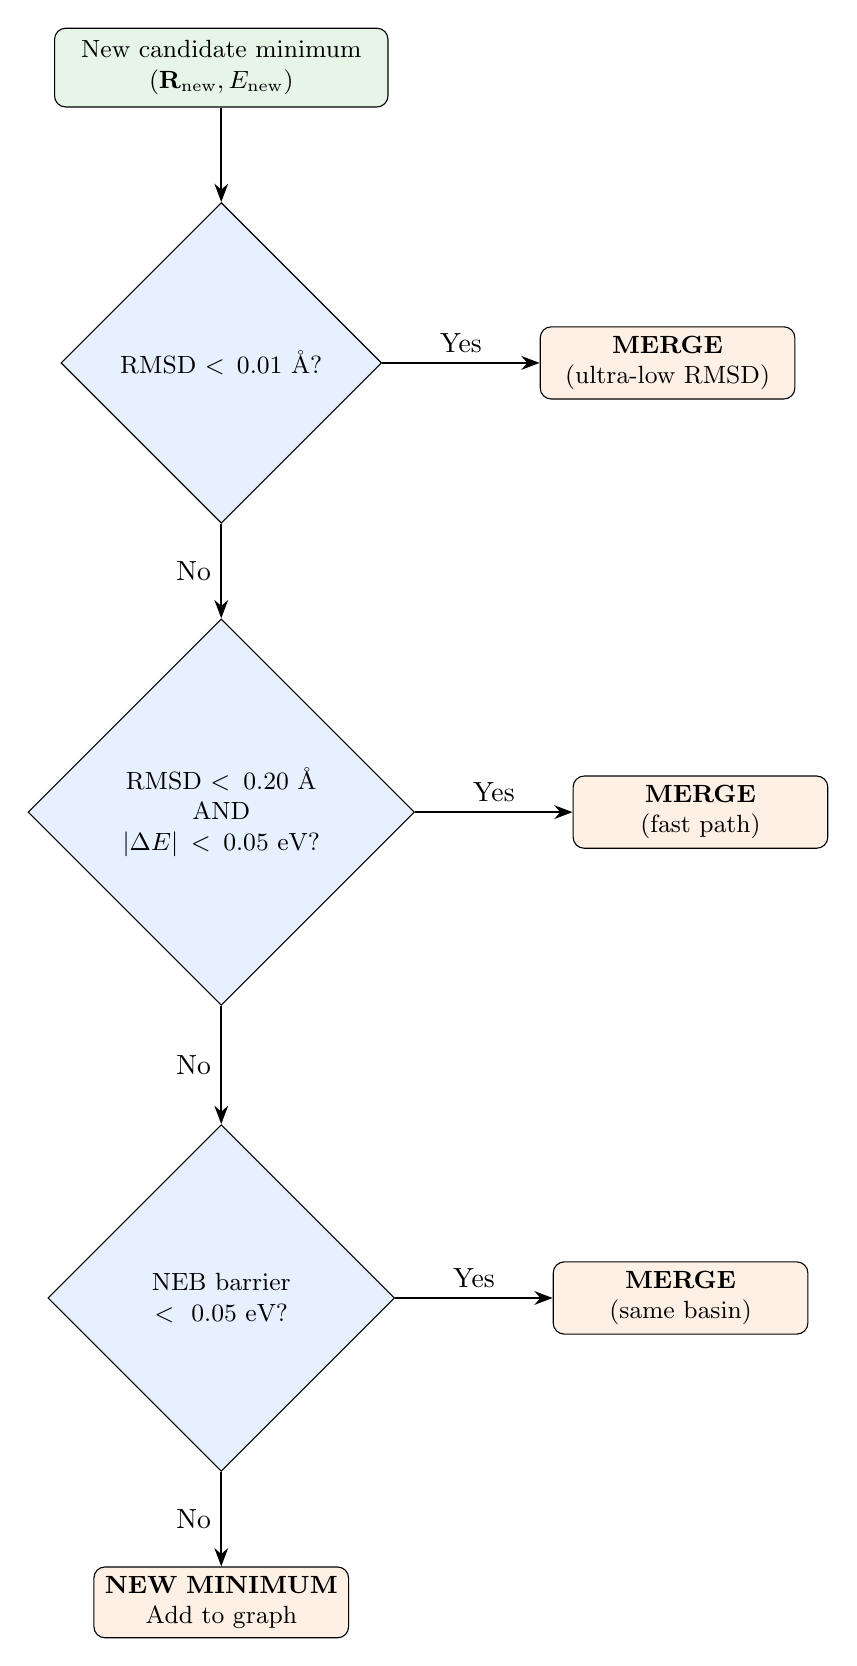
\begin{tikzpicture}[
    node distance=1.5cm,
    decision/.style={diamond, draw, fill=threshbox, text width=3.5cm, align=center, inner sep=2pt, font=\small},
    block/.style={rectangle, draw, fill=evalbox, text width=4cm, align=center, rounded corners, minimum height=1cm, font=\small},
    result/.style={rectangle, draw, fill=warnbox, text width=3cm, align=center, rounded corners, minimum height=0.8cm, font=\small},
    arrow/.style={-Stealth, thick},
]
    \node[block] (start) {New candidate minimum\\$(\mathbf{R}_\text{new}, E_\text{new})$};

    \node[decision, below=1.2cm of start] (tier1) {RMSD $< 0.01$~\AA?};

    \node[result, right=2cm of tier1] (merge1) {\textbf{MERGE}\\(ultra-low RMSD)};

    \node[decision, below=1.2cm of tier1] (tier2) {RMSD $< 0.20$~\AA\\AND\\$|\Delta E| < 0.05$~eV?};

    \node[result, right=2cm of tier2] (merge2) {\textbf{MERGE}\\(fast path)};

    \node[decision, below=1.5cm of tier2] (tier3) {NEB barrier\\$< 0.05$~eV?};

    \node[result, right=2cm of tier3] (merge3) {\textbf{MERGE}\\(same basin)};

    \node[result, below=1.2cm of tier3] (new) {\textbf{NEW MINIMUM}\\Add to graph};

    \draw[arrow] (start) -- (tier1);
    \draw[arrow] (tier1) -- node[above] {Yes} (merge1);
    \draw[arrow] (tier1) -- node[left] {No} (tier2);
    \draw[arrow] (tier2) -- node[above] {Yes} (merge2);
    \draw[arrow] (tier2) -- node[left] {No} (tier3);
    \draw[arrow] (tier3) -- node[above] {Yes} (merge3);
    \draw[arrow] (tier3) -- node[left] {No} (new);
\end{tikzpicture}
\caption{Three-tier deduplication flowchart for minima.}
\label{fig:dedup}
\end{figure}

\paragraph{Tier 1: Ultra-Low RMSD ($< \SI{0.01}{\angstrom}$).}
If the RMSD is below \SI{0.01}{\angstrom}, the structures are considered geometrically identical, and the candidate is merged \textbf{regardless of energy difference}. The rationale: at this level of geometric similarity, any energy difference is purely ML model noise.

\paragraph{Tier 2: RMSD + Energy Fast Path.}
If $\text{RMSD} < \SI{0.20}{\angstrom}$ \textbf{and} $|\Delta E| < \SI{0.05}{eV}$: merge without NEB. This handles the common case where the same minimum is found with slightly different geometries.

\paragraph{Tier 3: Nudged Elastic Band (NEB).}
For all remaining pairs (where the fast path didn't match), a \textbf{NEB calculation} is performed to check whether the two structures are in the same energy basin (Section~\ref{sec:neb}).

\begin{threshbox}
\begin{tabular}{lrl}
\toprule
Tier & Threshold & Criterion \\
\midrule
1 (ultra-low) & RMSD $< 0.01$~\AA & Geometry only (ignore energy) \\
2 (fast) & RMSD $< 0.20$~\AA\ \textbf{and} $|\Delta E| < 0.05$~eV & Both must pass \\
3 (NEB) & Barrier $< 0.05$~eV & Definitive check \\
\bottomrule
\end{tabular}
\end{threshbox}

\textbf{Merge tracking:} When a minimum is merged, the existing minimum's \texttt{n\_merged} counter is incremented and the \texttt{max\_merge\_rmsd} is updated. This provides diagnostics about how many duplicates each minimum attracts and at what RMSD.

\subsection{Batched Deduplication}

When multiple new minima are found simultaneously (from validating multiple TSs in one exploration step), a \textbf{batched} deduplication procedure is used:

\begin{enumerate}
    \item \textbf{Stage 1a:} Fast RMSD scan of all new candidates against all existing minima.
    \item \textbf{Stage 1b:} Batched NEB for unresolved pairs (all NEB bands run in a single GPU call per FIRE step, giving $\sim$$70\times$ speedup over sequential NEB).
    \item \textbf{Stage 2a:} Fast RMSD cross-check of surviving new candidates against each other.
    \item \textbf{Stage 2b:} Batched NEB cross-check for remaining pairs.
    \item \textbf{Materialize:} Add unique minima to graph, resolve cross-references.
\end{enumerate}

\begin{evaluation}
The three-tier deduplication is well-designed from a computational chemistry perspective:

\begin{itemize}
    \item \textbf{Tier 1 (\SI{0.01}{\angstrom}):} At this RMSD, the structures are essentially superimposable---less than 1\% of a bond length. The energy can differ only due to numerical noise in the ML model. Ignoring the energy here is correct.

    \item \textbf{Tier 2 (\SI{0.20}{\angstrom} + \SI{0.05}{eV}):} An RMSD of \SI{0.20}{\angstrom} is small---about the amplitude of a low-frequency vibration at room temperature. Combined with the energy gate of \SI{0.05}{eV} ($\approx$ \SI{1.15}{kcal/mol}, which is $\sim 2\,k_BT$ at \SI{300}{K}), this catches structures that are thermally accessible variants of the same minimum. The dual criterion (both must pass) prevents merging structures that happen to have similar geometry but very different energies (which would indicate they're in different basins despite geometric similarity).

    \item \textbf{Tier 3 (NEB with \SI{0.05}{eV} barrier):} This is the definitive test. Two structures are in the same basin if and only if there is no significant barrier between them. A threshold of \SI{0.05}{eV} ($\approx$ \SI{1.15}{kcal/mol} $\approx 2\,k_BT$) means that any barrier smaller than thermal energy is considered ``no barrier''---the system can freely interconvert between the two structures at room temperature.
\end{itemize}

\textbf{Key concern:} The NEB runs against \emph{all} existing minima, not just geometrically similar ones. For large graphs with hundreds of minima, this could be expensive. The code mitigates this with batched GPU evaluation, but it scales as $O(N_\text{existing})$ per new minimum. In practice, the number of minima for a single molecule's conformational PES is typically $O(10)$--$O(100)$, so this should be manageable.

\textbf{The \SI{0.05}{eV} NEB barrier threshold is aggressive.} Some conformational interconversions (e.g., ring flips, amide rotations) have barriers around \SI{0.05}--\SI{0.2}{eV}. At the \SI{0.05}{eV} threshold, these would be considered ``same basin,'' which merges distinct conformers. Whether this is desirable depends on the application---for kinetic modeling at room temperature, these interconversions are indeed fast, so merging is justified. For cryogenic or gas-phase studies, this would lose relevant information.
\end{evaluation}


%=============================================================================
\section{Nudged Elastic Band (NEB)}
\label{sec:neb}
%=============================================================================

The NEB method is used exclusively for deduplication: determining whether two minima are in the same energy basin. The implementation follows the improved tangent method of Henkelman \& J\'{o}nsson (2000).

\subsection{Band Construction}

\begin{enumerate}
    \item The two endpoint structures are optimally aligned (Kabsch + permutation, Section~\ref{sec:rmsd}).
    \item The number of interior images is adaptive: $N = \max(5, \min(12, \lceil \text{RMSD}/0.15 \rceil))$.
    \item Images are interpolated using the \textbf{IDPP} (Image-Dependent Pair Potential) method via ASE, which produces a physically reasonable initial band even for complex rearrangements.
\end{enumerate}

\subsection{Two-Phase Optimization}

\begin{enumerate}
    \item \textbf{Phase 1 (regular NEB):} 2/3 of the total FIRE steps. Relaxes all images onto the minimum energy path (MEP).
    \item \textbf{Early bail:} If the barrier after Phase 1 exceeds \SI{1.0}{eV}, the band is considered unphysical (bad interpolation). The check returns ``not same basin.''
    \item \textbf{Phase 2 (CI-NEB):} Remaining 1/3 of FIRE steps with climbing image enabled. The highest-energy image is pushed toward the true saddle point, refining the barrier estimate.
\end{enumerate}

\subsection{Same-Basin Criterion}

The barrier is computed as:
\begin{equation}
    \Delta E^\ddagger = \max_i(E_i) - \max(E_\text{endpoint 1}, E_\text{endpoint 2})
\end{equation}
i.e., the barrier above the \emph{higher} endpoint. If $\Delta E^\ddagger < \SI{0.05}{eV}$, the two structures are in the same basin.

\begin{threshbox}
\begin{tabular}{lrl}
\toprule
Parameter & Default & Description \\
\midrule
\texttt{neb\_fire\_steps} & 150 & Total FIRE optimization steps \\
\texttt{neb\_n\_images} & 5--12 & Interior images (adaptive) \\
\texttt{neb\_spring\_constant} & \SI{0.1}{eV/\angstrom^2} & Spring constant \\
\texttt{neb\_barrier\_threshold} & \SI{0.05}{eV} & Same-basin cutoff \\
Phase 1 early bail & \SI{1.0}{eV} & Abort if barrier too high \\
NEB convergence & \SI{0.05}{eV/\angstrom} & Max NEB force for convergence \\
\bottomrule
\end{tabular}
\end{threshbox}

\begin{evaluation}
The two-phase NEB approach (regular $\to$ CI-NEB) is important and well-justified. Running CI-NEB from the start can cause the climbing image to be pushed to an absurdly high energy if the initial interpolation is poor. Stabilizing the band first with regular NEB and then refining with CI-NEB is standard best practice.

The adaptive number of images ($\lceil\text{RMSD}/0.15\rceil$, clamped to [5, 12]) is a nice touch: more images for larger structural changes ensures adequate resolution of the MEP, while capping at 12 prevents excessive computational cost.

The spring constant of \SI{0.1}{eV/\angstrom^2} is moderate---stiff enough to keep images evenly spaced but not so stiff that image-image interactions dominate over the true PES forces.

\textbf{The 150 FIRE steps may be insufficient for complex rearrangements.} NEB convergence can be slow, especially for long reaction paths or when the MEP has sharp turns. However, since NEB is used here only for a binary same-basin/different-basin classification (not for accurate barrier determination), full convergence is not strictly necessary---an approximate barrier estimate is sufficient.
\end{evaluation}


%=============================================================================
\section{Transition State Deduplication}
\label{sec:ts-dedup}
%=============================================================================

When adding a new TS to the graph, it is compared against existing TSs that connect the \textbf{same pair of endpoints}. The deduplication uses multiple criteria:

\begin{enumerate}
    \item \textbf{Same endpoints:} The TS must connect the same pair of minima (in either orientation).
    \item \textbf{Ultra-low RMSD ($< \SI{0.01}{\angstrom}$):} Identical TS, always merge.
    \item \textbf{Barrier-profile match:} If the forward and backward barriers match within \SI{0.1}{eV} (checking both orientations):
    \begin{align}
        |B_\text{fwd}^\text{new} - B_\text{fwd}^\text{old}| &< \SI{0.1}{eV} \;\textbf{and}\; |B_\text{bwd}^\text{new} - B_\text{bwd}^\text{old}| < \SI{0.1}{eV} \notag \\
        \textbf{or}\quad |B_\text{fwd}^\text{new} - B_\text{bwd}^\text{old}| &< \SI{0.1}{eV} \;\textbf{and}\; |B_\text{bwd}^\text{new} - B_\text{fwd}^\text{old}| < \SI{0.1}{eV}
    \end{align}
    This catches the same saddle point found from different MD trajectories.
    \item \textbf{Standard RMSD + energy:} RMSD $< \SI{0.20}{\angstrom}$ and $|\Delta E| < \SI{0.05}{eV}$.
\end{enumerate}

\begin{evaluation}
The barrier-profile deduplication is an important addition beyond simple geometric comparison. Two TSs connecting the same pair of minima with the same barrier heights ($\pm\SI{0.1}{eV}$) are almost certainly the same saddle point---even if the geometric RMSD is somewhat larger than the threshold (e.g., due to a floppy substituent).

The \SI{0.1}{eV} barrier tolerance is quite generous ($\approx\SI{2.3}{kcal/mol}$), which means that TSs with noticeably different barrier heights could be merged. This is probably acceptable for ML-level accuracy but could mask genuinely distinct reaction pathways with similar barriers. For high-accuracy studies, tightening this to \SI{0.05}{eV} might be warranted.

Note that TS deduplication only applies when endpoints match---TSs connecting different pairs of minima are never compared, even if they happen to have similar geometries. This is correct because a saddle point is defined by its connectivity (which basins it connects), not just its geometry.
\end{evaluation}


%=============================================================================
\section{Complete Threshold Reference}
\label{sec:thresholds}
%=============================================================================

\begin{longtable}{p{5cm}rlp{6cm}}
\toprule
\textbf{Parameter} & \textbf{Value} & \textbf{Unit} & \textbf{Where Used} \\
\midrule
\endfirsthead
\toprule
\textbf{Parameter} & \textbf{Value} & \textbf{Unit} & \textbf{Where Used} \\
\midrule
\endhead
\bottomrule
\endfoot
\multicolumn{4}{l}{\textbf{Molecular Dynamics}} \\
\midrule
MD steps & 2500 & steps & PES exploration MD \\
MD timestep & 0.5 & fs & Integration \\
Temperature & 300 & K & Langevin thermostat \\
Thermostat $\tau$ & 100 & fs & Langevin coupling \\
Save interval & 10 & steps & Trajectory snapshots \\
\midrule
\multicolumn{4}{l}{\textbf{TS Candidate Selection}} \\
\midrule
Candidates per iteration & 32 & -- & Random or saddle metric \\
Saddle metric percentile & 10 & \% & Top frames if metric used \\
\midrule
\multicolumn{4}{l}{\textbf{P-RFO Saddle Optimization}} \\
\midrule
Max steps & 120 & steps & Per candidate \\
Force max tolerance & 0.01 & eV/\AA & Convergence criterion \\
Force RMS tolerance & 0.005 & eV/\AA & Convergence criterion \\
Initial trust radius & 0.5 & \AA & Step constraint \\
Min trust radius & 0.01 & \AA & Floor for adaptive trust \\
Max trust radius & 0.3 & \AA & Ceiling for adaptive trust \\
TS trust scale & 1.5 & -- & TS mode gets $1.5\times$ \\
Step accept $\rho$ & 0.1 & -- & Min ratio to accept \\
Max retries/step & 5 & -- & Before accepting anyway \\
Early stop window & 20 & steps & For stuck/oscillation check \\
Early stop displacement & $10^{-4}$ & \AA & Min net displacement \\
Early stop efficiency & 0.1 & -- & Min net/path ratio \\
\midrule
\multicolumn{4}{l}{\textbf{TS Validation (IRC)}} \\
\midrule
Eigenvalue threshold & $-0.01$ & eV/\AA$^2$ & Min curvature for TS \\
Adaptive displacement & $\sqrt{0.16/|\lambda|}$ & \AA & Along imaginary mode \\
Min displacement & 0.02 & \AA & Clamp lower bound \\
Max displacement & 0.5 & \AA & Clamp upper bound \\
Energy threshold (both sides) & 0.04 & eV & Endpoints below TS \\
Energy threshold (one side) & 0.005 & eV & Relaxed asymmetric \\
Min endpoint RMSD & 0.25 & \AA & Endpoints must differ \\
Relaxation force max & 0.005 & eV/\AA & IRC endpoint convergence \\
Relaxation max steps & 120 & steps & IRC relaxation \\
\midrule
\multicolumn{4}{l}{\textbf{Minimum Deduplication}} \\
\midrule
Ultra-low RMSD & 0.01 & \AA & Always merge (Tier 1) \\
RMSD threshold & 0.20 & \AA & Fast merge (Tier 2) \\
Energy threshold & 0.05 & eV & Fast merge (Tier 2) \\
NEB barrier threshold & 0.05 & eV & Same-basin (Tier 3) \\
\midrule
\multicolumn{4}{l}{\textbf{NEB}} \\
\midrule
Interior images & 5--12 & -- & Adaptive on RMSD \\
FIRE steps & 150 & steps & Total (100 reg + 50 CI) \\
Spring constant & 0.1 & eV/\AA$^2$ & Image coupling \\
Phase 1 bail threshold & 1.0 & eV & Abort unphysical band \\
Force convergence & 0.05 & eV/\AA & Max NEB force \\
\midrule
\multicolumn{4}{l}{\textbf{TS Deduplication}} \\
\midrule
Ultra-low RMSD & 0.01 & \AA & Same TS \\
Barrier tolerance & 0.1 & eV & Same saddle, different trajectory \\
RMSD threshold & 0.20 & \AA & Standard dedup \\
Energy threshold & 0.05 & eV & Standard dedup \\
\midrule
\multicolumn{4}{l}{\textbf{Hessian Eigenvalue Thresholds}} \\
\midrule
Zero-mode masking & $10^{-5}$ & eV/\AA$^2$ & Filter translation/rotation \\
Negative eigenvalue reporting & $5\times10^{-3}$ & eV/\AA$^2$ & Count negative eigs \\
Negative eigenvalue detection & $10^{-4}$ & eV/\AA$^2$ & Find imaginary modes \\
\end{longtable}


%=============================================================================
\section{Batched GPU Computation}
\label{sec:batching}
%=============================================================================

A critical implementation detail: all computationally expensive operations (Hessians, force/energy evaluations for NEB, P-RFO trial steps) are \textbf{batched across multiple structures} and evaluated in a single GPU call. This means:

\begin{itemize}
    \item All 32 P-RFO saddle searches run in lockstep: at each step, all active searches get their Hessian in one GPU call, each computes its step on CPU, then all trial energies are evaluated in one GPU call.
    \item NEB bands for deduplication: all interior images across all NEB bands are batched into a single force evaluation per FIRE step.
    \item TS validation: all displaced geometries (2 per valid TS) are relaxed in parallel.
\end{itemize}

This batching is what makes the algorithm practical on GPU hardware. Without it, evaluating 32 saddle searches $\times$ 120 steps $\times$ 2 GPU calls/step = 7680 individual GPU calls would dominate the runtime.

\begin{evaluation}
The batched approach is computationally efficient and doesn't compromise chemical accuracy---the same calculation is performed regardless of whether structures are evaluated one-by-one or in a batch. The lockstep P-RFO approach means that the batch shrinks as individual searches converge or early-stop, but the overhead of carrying unconverged searches is minimal because they all share the same GPU call.
\end{evaluation}


%=============================================================================
\section{Overall Assessment}
\label{sec:assessment}
%=============================================================================

\begin{evaluation}
\textbf{Summary of chemical soundness:}

\begin{enumerate}
    \item \textbf{The overall workflow is chemically sound.} MD sampling $\to$ saddle optimization $\to$ IRC validation $\to$ deduplication follows established methodology for automated PES exploration.

    \item \textbf{The P-RFO implementation is correct} and includes important practical features (mode-following, adaptive trust, partitioned trust radii for TS vs.\ minimization directions).

    \item \textbf{The TS validation is rigorous.} Requiring both endpoints to be lower than the TS, checking for structural distinctness via RMSD, and using the full Hessian eigenvalue spectrum are all correct chemical criteria.

    \item \textbf{The deduplication is thorough.} The three-tier approach (geometric $\to$ geometric+energetic $\to$ NEB) is both efficient and reliable. The NEB-based same-basin check is the gold standard.

    \item \textbf{Key thresholds are reasonable for ML force fields.} The force tolerance (\SI{0.01}{eV/\angstrom}), RMSD threshold (\SI{0.20}{\angstrom}), and energy threshold (\SI{0.05}{eV}) all reflect the expected accuracy of current ML potentials.
\end{enumerate}

\textbf{Points for the computational chemist to verify:}

\begin{enumerate}
    \item \textbf{ML Hessian quality:} The entire TS finding and validation pipeline depends on accurate Hessians. If the ML model produces noisy Hessians (spurious negative eigenvalues, incorrect curvature), the algorithm will produce false positives (non-TS structures classified as TSs) or false negatives (real TSs rejected). Spot-checking Hessian eigenvalues against DFT for representative cases is recommended.

    \item \textbf{NEB barrier threshold of \SI{0.05}{eV}:} This determines what counts as a ``distinct'' minimum. At \SI{300}{K}, $k_BT \approx \SI{0.026}{eV}$, so \SI{0.05}{eV} $\approx 2\,k_BT$. Any barrier below this will be freely crossed at room temperature, making the merging defensible for kinetic modeling. But for low-temperature applications or entropy-sensitive processes, this may be too aggressive.

    \item \textbf{Asymmetric TS validation (\SI{0.005}{eV}):} The one-side relaxed threshold is very close to model noise. Monitor how often this criterion is the deciding factor---if frequently, it may be admitting questionable TSs.

    \item \textbf{Lowest-energy-first exploration:} This biases toward thermodynamically stable regions. If high-energy reaction channels are of interest, consider supplementing with random or connectivity-based selection.

    \item \textbf{Single conformer per basin:} The algorithm merges all structures within a basin into a single representative minimum. The energy of the representative is the energy of the \emph{first} structure found (not necessarily the lowest-energy conformer within that basin). If conformational averaging is important, this should be verified.
\end{enumerate}
\end{evaluation}

\begin{concern}
\textbf{All energies, forces, and Hessians come from an ML force field, not quantum chemistry.} While this enables the exploration of a vast number of structures, the results should be validated with DFT or higher-level methods for any reaction that will be used quantitatively (e.g., for computing rate constants). The CRN-Cloud system does include a DFT refinement step (PBE0/def2-TZVPP single-points) downstream, but the \emph{selection} of which TSs and minima enter the reaction network is based entirely on ML predictions. An ML model that systematically underestimates barriers for a certain reaction type could miss relevant chemistry, and one that systematically overestimates could include spurious reactions. Cross-validation against DFT for a representative subset is essential.
\end{concern}


%=============================================================================
\section{Appendix: Order of Operations Summary}
%=============================================================================

For reference, the complete order of operations within a single exploration iteration:

\begin{enumerate}[leftmargin=2cm]
    \item[\textbf{1.}] \textbf{Select} lowest-energy unexplored minimum.
    \item[\textbf{2.}] \textbf{MD simulation:} 2500 steps, Langevin at \SI{300}{K}, \SI{0.5}{fs} timestep $\to$ 250 frames.
    \item[\textbf{3.}] \textbf{Sample} 32 candidate frames (random or saddle metric).
    \item[\textbf{4.}] \textbf{Batched P-RFO:} Optimize all 32 candidates toward saddle points (up to 120 steps each, batched GPU).
    \item[\textbf{5.}] \textbf{Filter:} Keep only converged first-order saddle points (force $< \SI{0.01}{eV/\angstrom}$, exactly 1 negative eigenvalue).
    \item[\textbf{6.}] \textbf{Batched TS validation:}
    \begin{enumerate}[label=\alph*.]
        \item Compute Hessian at each TS (batched GPU).
        \item Check eigenvalue $< -\SI{0.01}{eV/\angstrom^2}$.
        \item Compute adaptive displacement along imaginary mode.
        \item Generate $2 \times N_\text{valid}$ displaced geometries ($\pm$ direction).
        \item Batched Newton relaxation of all displaced geometries (batched GPU, up to 120 steps).
        \item Check energy criterion: both endpoints $> \SI{0.04}{eV}$ below TS (or asymmetric $0.04/0.005$).
        \item Check RMSD criterion: endpoints differ by $> \SI{0.25}{\angstrom}$.
    \end{enumerate}
    \item[\textbf{7.}] \textbf{Batched endpoint deduplication:}
    \begin{enumerate}[label=\alph*.]
        \item Canonicalize all endpoint positions (RDKit atom ordering).
        \item Fast RMSD scan vs.\ existing minima ($< \SI{0.20}{\angstrom}$ and $< \SI{0.05}{eV}$ $\to$ merge).
        \item Batched NEB for remaining pairs (barrier $< \SI{0.05}{eV}$ $\to$ same basin).
        \item Cross-check new endpoints against each other (same criteria).
        \item Add unique new minima to graph.
    \end{enumerate}
    \item[\textbf{8.}] \textbf{Add TSs to graph:}
    \begin{enumerate}[label=\alph*.]
        \item Compute barriers from relaxation trajectories (force integration) or endpoint energies.
        \item Check for duplicate TSs (same endpoints + barrier profile within \SI{0.1}{eV}, or RMSD $< \SI{0.20}{\angstrom}$).
        \item Add new TSs as edges in the graph.
    \end{enumerate}
    \item[\textbf{9.}] \textbf{Mark} current minimum as explored.
    \item[\textbf{10.}] \textbf{Save} checkpoint to disk.
    \item[\textbf{11.}] \textbf{Repeat} from Step 1.
\end{enumerate}


\end{document}
